% Options for packages loaded elsewhere
\PassOptionsToPackage{unicode,linktoc=all}{hyperref}
\PassOptionsToPackage{hyphens}{url}
\PassOptionsToPackage{dvipsnames,svgnames,x11names}{xcolor}
%
\documentclass[
  a4paper,
]{article}
\usepackage{amsmath,amssymb}
\usepackage{iftex}
\ifPDFTeX
  \usepackage[T1]{fontenc}
  \usepackage[utf8]{inputenc}
  \usepackage{textcomp} % provide euro and other symbols
\else % if luatex or xetex
  \usepackage{unicode-math} % this also loads fontspec
  \defaultfontfeatures{Scale=MatchLowercase}
  \defaultfontfeatures[\rmfamily]{Ligatures=TeX,Scale=1}
\fi
\usepackage{lmodern}
\ifPDFTeX\else
  % xetex/luatex font selection
\fi
% Use upquote if available, for straight quotes in verbatim environments
\IfFileExists{upquote.sty}{\usepackage{upquote}}{}
\IfFileExists{microtype.sty}{% use microtype if available
  \usepackage[]{microtype}
  \UseMicrotypeSet[protrusion]{basicmath} % disable protrusion for tt fonts
}{}
\makeatletter
\@ifundefined{KOMAClassName}{% if non-KOMA class
  \IfFileExists{parskip.sty}{%
    \usepackage{parskip}
  }{% else
    \setlength{\parindent}{0pt}
    \setlength{\parskip}{6pt plus 2pt minus 1pt}}
}{% if KOMA class
  \KOMAoptions{parskip=half}}
\makeatother
\usepackage{xcolor}
\usepackage[margin=25mm]{geometry}
\usepackage{color}
\usepackage{fancyvrb}
\newcommand{\VerbBar}{|}
\newcommand{\VERB}{\Verb[commandchars=\\\{\}]}
\DefineVerbatimEnvironment{Highlighting}{Verbatim}{commandchars=\\\{\}}
% Add ',fontsize=\small' for more characters per line
\usepackage{framed}
\definecolor{shadecolor}{RGB}{48,48,48}
\newenvironment{Shaded}{\begin{snugshade}}{\end{snugshade}}
\newcommand{\AlertTok}[1]{\textcolor[rgb]{1.00,0.81,0.69}{#1}}
\newcommand{\AnnotationTok}[1]{\textcolor[rgb]{0.50,0.62,0.50}{\textbf{#1}}}
\newcommand{\AttributeTok}[1]{\textcolor[rgb]{0.80,0.80,0.80}{#1}}
\newcommand{\BaseNTok}[1]{\textcolor[rgb]{0.86,0.64,0.64}{#1}}
\newcommand{\BuiltInTok}[1]{\textcolor[rgb]{0.80,0.80,0.80}{#1}}
\newcommand{\CharTok}[1]{\textcolor[rgb]{0.86,0.64,0.64}{#1}}
\newcommand{\CommentTok}[1]{\textcolor[rgb]{0.50,0.62,0.50}{#1}}
\newcommand{\CommentVarTok}[1]{\textcolor[rgb]{0.50,0.62,0.50}{\textbf{#1}}}
\newcommand{\ConstantTok}[1]{\textcolor[rgb]{0.86,0.64,0.64}{\textbf{#1}}}
\newcommand{\ControlFlowTok}[1]{\textcolor[rgb]{0.94,0.87,0.69}{#1}}
\newcommand{\DataTypeTok}[1]{\textcolor[rgb]{0.87,0.87,0.75}{#1}}
\newcommand{\DecValTok}[1]{\textcolor[rgb]{0.86,0.86,0.80}{#1}}
\newcommand{\DocumentationTok}[1]{\textcolor[rgb]{0.50,0.62,0.50}{#1}}
\newcommand{\ErrorTok}[1]{\textcolor[rgb]{0.76,0.75,0.62}{#1}}
\newcommand{\ExtensionTok}[1]{\textcolor[rgb]{0.80,0.80,0.80}{#1}}
\newcommand{\FloatTok}[1]{\textcolor[rgb]{0.75,0.75,0.82}{#1}}
\newcommand{\FunctionTok}[1]{\textcolor[rgb]{0.94,0.94,0.56}{#1}}
\newcommand{\ImportTok}[1]{\textcolor[rgb]{0.80,0.80,0.80}{#1}}
\newcommand{\InformationTok}[1]{\textcolor[rgb]{0.50,0.62,0.50}{\textbf{#1}}}
\newcommand{\KeywordTok}[1]{\textcolor[rgb]{0.94,0.87,0.69}{#1}}
\newcommand{\NormalTok}[1]{\textcolor[rgb]{0.80,0.80,0.80}{#1}}
\newcommand{\OperatorTok}[1]{\textcolor[rgb]{0.94,0.94,0.82}{#1}}
\newcommand{\OtherTok}[1]{\textcolor[rgb]{0.94,0.94,0.56}{#1}}
\newcommand{\PreprocessorTok}[1]{\textcolor[rgb]{1.00,0.81,0.69}{\textbf{#1}}}
\newcommand{\RegionMarkerTok}[1]{\textcolor[rgb]{0.80,0.80,0.80}{#1}}
\newcommand{\SpecialCharTok}[1]{\textcolor[rgb]{0.86,0.64,0.64}{#1}}
\newcommand{\SpecialStringTok}[1]{\textcolor[rgb]{0.80,0.58,0.58}{#1}}
\newcommand{\StringTok}[1]{\textcolor[rgb]{0.80,0.58,0.58}{#1}}
\newcommand{\VariableTok}[1]{\textcolor[rgb]{0.80,0.80,0.80}{#1}}
\newcommand{\VerbatimStringTok}[1]{\textcolor[rgb]{0.80,0.58,0.58}{#1}}
\newcommand{\WarningTok}[1]{\textcolor[rgb]{0.50,0.62,0.50}{\textbf{#1}}}
\usepackage{longtable,booktabs,array}
\usepackage{calc} % for calculating minipage widths
% Correct order of tables after \paragraph or \subparagraph
\usepackage{etoolbox}
\makeatletter
\patchcmd\longtable{\par}{\if@noskipsec\mbox{}\fi\par}{}{}
\makeatother
% Allow footnotes in longtable head/foot
\IfFileExists{footnotehyper.sty}{\usepackage{footnotehyper}}{\usepackage{footnote}}
\makesavenoteenv{longtable}
\usepackage{graphicx}
\makeatletter
\def\maxwidth{\ifdim\Gin@nat@width>\linewidth\linewidth\else\Gin@nat@width\fi}
\def\maxheight{\ifdim\Gin@nat@height>\textheight\textheight\else\Gin@nat@height\fi}
\makeatother
% Scale images if necessary, so that they will not overflow the page
% margins by default, and it is still possible to overwrite the defaults
% using explicit options in \includegraphics[width, height, ...]{}
\setkeys{Gin}{width=\maxwidth,height=\maxheight,keepaspectratio}
% Set default figure placement to htbp
\makeatletter
\def\fps@figure{htbp}
\makeatother
\usepackage{svg}
\setlength{\emergencystretch}{3em} % prevent overfull lines
\providecommand{\tightlist}{%
  \setlength{\itemsep}{0pt}\setlength{\parskip}{0pt}}
\setcounter{secnumdepth}{-\maxdimen} % remove section numbering
\newlength{\cslhangindent}
\setlength{\cslhangindent}{1.5em}
\newlength{\csllabelwidth}
\setlength{\csllabelwidth}{3em}
\newlength{\cslentryspacingunit} % times entry-spacing
\setlength{\cslentryspacingunit}{\parskip}
\newenvironment{CSLReferences}[2] % #1 hanging-ident, #2 entry spacing
 {% don't indent paragraphs
  \setlength{\parindent}{0pt}
  % turn on hanging indent if param 1 is 1
  \ifodd #1
  \let\oldpar\par
  \def\par{\hangindent=\cslhangindent\oldpar}
  \fi
  % set entry spacing
  \setlength{\parskip}{#2\cslentryspacingunit}
 }%
 {}
\usepackage{calc}
\newcommand{\CSLBlock}[1]{#1\hfill\break}
\newcommand{\CSLLeftMargin}[1]{\parbox[t]{\csllabelwidth}{#1}}
\newcommand{\CSLRightInline}[1]{\parbox[t]{\linewidth - \csllabelwidth}{#1}\break}
\newcommand{\CSLIndent}[1]{\hspace{\cslhangindent}#1}
\ifLuaTeX
\usepackage[bidi=basic]{babel}
\else
\usepackage[bidi=default]{babel}
\fi
\babelprovide[main,import]{british}
% get rid of language-specific shorthands (see #6817):
\let\LanguageShortHands\languageshorthands
\def\languageshorthands#1{}
% $HOME/.pandoc/defaults/latex-header-includes.tex
% Common header includes for both lualatex and xelatex engines.
%
% Preliminaries
%
% \PassOptionsToPackage{rgb,dvipsnames,svgnames}{xcolor}
% \PassOptionsToPackage{main=british}{babel}
\PassOptionsToPackage{english}{selnolig}
\AtBeginEnvironment{quote}{\small}
\AtBeginEnvironment{quotation}{\small}
\AtBeginEnvironment{longtable}{\centering}
%
% Packages that are useful to include
%
\usepackage{graphicx}
\usepackage{subcaption}
\usepackage[inkscapeversion=1]{svg}
\usepackage[defaultlines=4,all]{nowidow}
\usepackage{etoolbox}
\usepackage{fontsize}
\usepackage{newunicodechar}
\usepackage{pdflscape}
\usepackage{fnpct}
\usepackage{parskip}
  \setlength{\parindent}{0pt}
\usepackage[style=american]{csquotes}
% \usepackage{setspace} Use the <fontname-plus.tex> files for setspace
%
\usepackage{hyperref} % cleveref must come AFTER hyperref
\usepackage[capitalize,noabbrev]{cleveref} % Must come after hyperref
\let\longdivision\relax
\usepackage{longdivision}
% noto-plus.tex
% Font-setting header file for use with Pandoc Markdown
% to generate PDF via LuaLaTeX.
% The main font is Noto Serif.
% Other main fonts are also available in appropriately named file.
\usepackage{fontspec}
\usepackage{setspace}
\setstretch{1.3}
%
\defaultfontfeatures{Ligatures=TeX,Scale=MatchLowercase,Renderer=Node} % at the start always
%
% For English
% See also https://tex.stackexchange.com/questions/574047/lualatex-amsthm-polyglossia-charissil-error
% We use Node as Renderer for the Latin Font and Greek Font and HarfBuzz as renderer ofr Indic fonts.
%
\babelfont{rm}[Script=Latin,Scale=1]{NotoSerif}% Config is at $HOME/texmf/tex/latex/NotoSerif.fontspec
\babelfont{sf}[Script=Latin]{SourceSansPro}% Config is at $HOME/texmf/tex/latex/SourceSansPro.fontspec
\babelfont{tt}[Script=Latin]{FiraMono}% Config is at $HOME/texmf/tex/latex/FiraMono.fontspec
%
% Sanskrit, Tamil, and Greek fonts
%
\babelprovide[import, onchar=ids fonts]{sanskrit}
\babelprovide[import, onchar=ids fonts]{tamil}
\babelprovide[import, onchar=ids fonts]{greek}
%
\babelfont[sanskrit]{rm}[Scale=1.1,Renderer=HarfBuzz,Script=Devanagari]{NotoSerifDevanagari}
\babelfont[sanskrit]{sf}[Scale=1.1,Renderer=HarfBuzz,Script=Devanagari]{NotoSansDevanagari}
\babelfont[tamil]{rm}[Renderer=HarfBuzz,Script=Tamil]{NotoSerifTamil}
\babelfont[tamil]{sf}[Renderer=HarfBuzz,Script=Tamil]{NotoSansTamil}
\babelfont[greek]{rm}[Script=Greek]{GentiumBookPlus}
%
% Math font
%
\usepackage{unicode-math} % seems not to hurt % fallabck
\setmathfont[bold-style=TeX]{STIX Two Math}
\usepackage{amsmath}
\usepackage{esdiff} % for derivative symbols
% \renewcommand{\mathbf}{\symbf}
%
%
% Other fonts
%
\newfontfamily{\emojifont}{Symbola}
%

\usepackage{titling}
\usepackage{fancyhdr}
    \pagestyle{fancy}
    \fancyhead{}
    \fancyfoot{}
    \renewcommand{\headrulewidth}{0.2pt}
    \renewcommand{\footrulewidth}{0.2pt}
    \fancyhead[LO,RE]{\scshape\thetitle}
    \fancyfoot[CO,CE]{\footnotesize Copyright © 2006\textendash\the\year, R (Chandra) Chandrasekhar}
    \fancyfoot[RE,RO]{\thepage}
%
\usepackage{newunicodechar}
\newunicodechar{√}{\textsf{√}}
\ifLuaTeX
  \usepackage{selnolig}  % disable illegal ligatures
\fi
\IfFileExists{bookmark.sty}{\usepackage{bookmark}}{\usepackage{hyperref}}
\IfFileExists{xurl.sty}{\usepackage{xurl}}{} % add URL line breaks if available
\urlstyle{sf}
\hypersetup{
  pdftitle={Using Typst for Letters},
  pdfauthor={R (Chandra) Chandrasekhar},
  pdflang={en-GB},
  colorlinks=true,
  linkcolor={DarkOliveGreen},
  filecolor={Purple},
  citecolor={DarkKhaki},
  urlcolor={Maroon},
  pdfcreator={LaTeX via pandoc}}

\title{Using \texttt{Typst} for Letters}
\author{R (Chandra) Chandrasekhar}
\date{2024-01-01 | 2024-01-08}

\begin{document}
\maketitle

\thispagestyle{empty}


\hypertarget{the-road-from-latex-to-typst}{%
\subsection{The road from LaTeX to
Typst}\label{the-road-from-latex-to-typst}}

Despite the ubiquity of emails, each of us has had to write a letter to
someone at some time in our lives. In the days of
\href{https://www.merriam-webster.com/dictionary/snail\%20mail}{snail
mail}, we used to write by hand, using lightweight paper---specially
made for conveying the maximum information for the least weight of paper
plus envelope---to minimize postage charges. Those days are well and
truly behind us now, to the extent that many of us rarely lift a pencil
or put pen to paper, except to sign our names or make some perfunctory
calculation.

After the dedicated but computationally wasteful
\href{https://www.webopedia.com/definitions/word-processor/}{word
processor} was replaced by the general purpose personal computer, it was
but a short hop, step, and jump for the PC to simulate a word processor,
among its innumerable masquerades, to satisfy our need to be connected.

The advent of the \href{https://www.latex-project.org/}{LaTeX}
typesetting system was yet another boon for those of us who laboured,
with scissors, typed manuscripts, and pasted photographs, to publish
papers in learned journals, especially in fields requiring mathematics,
like science and engineering.

Nevertheless, I have always been dismayed by how cumbersome it has been
to typeset a simple letter using LaTeX. One has to jump deftly through
numerous hoops to get a decent-looking letter, even with the formidable
resources of LaTeX.

So, I was eager with anticipation when I first stumbled upon
\href{https://typst.app/}{\texttt{Typst}}
{[}\protect\hyperlink{ref-typst01}{1},\protect\hyperlink{ref-typst02}{2}{]},
which exhorted one to ``Compose papers/theses faster''. The
\href{https://github.com/typst/typst}{Typst home page} claims it is a
``A new markup-based typesetting system that is powerful and easy to
learn.'' Piqued by these promising assertions, I decided to take the
plunge with Typst, for the specific but express purpose of writing
letters. I have chronicled my experiences here.

\hypertarget{a-glancing-encounter-with-latex3}{%
\subsection{A glancing encounter with
LaTeX3}\label{a-glancing-encounter-with-latex3}}

I have been using LaTeX to write papers, theses, and books for well nigh
thirty years. Thus, I am a beneficiary of the LaTeX ecosystem, and can
vouch that the results from it are superior to those from a widely used
proprietary ``word processing'' program which shall remain unnamed.

Despite that, I was somewhat aghast when I saw how the new, experimental
LaTeX3 ``dialect'' or ``macro language'', or whatever it is called,
looked like. It is the successor to the ``LaTeX2ɛ'' we use now, and
while it might not impact end users much, it will certainly impinge upon
customizability. The code fragment below is taken from a blog entitled
``LaTeX3: Programming in LaTeX with Ease''
{[}\protect\hyperlink{ref-xiang2020}{3}{]}, and boy, did it make me
uneasy, even to gaze upon it, let alone attempt to understand it:

\begin{Shaded}
\begin{Highlighting}[]
\FunctionTok{\textbackslash{}ExplSyntaxOn}
\CommentTok{\% put the title in \textbackslash{}l\_tmpa\_tl}
\FunctionTok{\textbackslash{}tl}\NormalTok{\_set:Nn }\FunctionTok{\textbackslash{}l}\NormalTok{\_tmpa\_tl \{My\textasciitilde{}Title\}}
\CommentTok{\% construct the command in \textbackslash{}l\_tmpb\_tl}
\FunctionTok{\textbackslash{}tl}\NormalTok{\_set:Nx }\FunctionTok{\textbackslash{}l}\NormalTok{\_tmpb\_tl \{}\FunctionTok{\textbackslash{}exp}\NormalTok{\_not:N }\KeywordTok{\textbackslash{}section*}\NormalTok{ \{}\FunctionTok{\textbackslash{}l}\NormalTok{\_tmpa\_tl\}\}}
\FunctionTok{\textbackslash{}cs}\NormalTok{\_meaning:N }\FunctionTok{\textbackslash{}l}\NormalTok{\_tmpb\_tl }\CommentTok{\% macro:{-}\textgreater{}\textbackslash{}section *\{My Title\}}
\CommentTok{\% place the content of \textbackslash{}l\_tmpb\_tl into the input stream}
\FunctionTok{\textbackslash{}tl}\NormalTok{\_use:N }\FunctionTok{\textbackslash{}l}\NormalTok{\_tmpb\_tl}
\FunctionTok{\textbackslash{}ExplSyntaxOff}
\end{Highlighting}
\end{Shaded}

If you are as put off as I was by the code above, we are already on the
same page. If you are a diehard LaTeX
\href{https://www.collinsdictionary.com/dictionary/hindi-english/\%E0\%A4\%AD\%E0\%A4\%95\%E0\%A5\%8D\%E0\%A4\%A4}{bhakt},
you are unlikely to be swayed by what I have to say, and might as well
stop reading now. If you are a fence-sitter, read along and make up your
mind at the end.

\hypertarget{the-pandoc-markdown-duo}{%
\subsection{The Pandoc-Markdown duo}\label{the-pandoc-markdown-duo}}

By the time these blogs were written, I had already started using
\href{https://pandoc.org/}{Pandoc} and its extended
\href{https://pandoc.org/chunkedhtml-demo/8-pandocs-markdown.html}{Markdown}
in much of what I wrote. They are an efficient duo, and with the help of
LaTeX, I have been able to produce a PDF document that bears more than a
passing similarity to the HTML5 blog originally generated from Markdown
using Pandoc.

So, all was smooth sailing, until I needed to write letters, and was
that experience ugly! Suffice it to say that letter writing was not on
the minds of most document typesetting designers when they
\href{https://www.thefreedictionary.com/ideated}{ideated} their
creations.

\hypertarget{the-attractions-of-typst}{%
\subsection{The attractions of Typst}\label{the-attractions-of-typst}}

Like LaTeX, Typst is a markup-based programmable typesetting system. But
it is fast and easy to use. Typst provides easy customizability because
the programming syntax used in scripting is human-readable. Sensibly, it
acts on objects that have meaning in the context of a document. It
affects both the structure and content of a document. Like LaTeX, it
produces PDF, which is bound to paper sizes. Should Typst also provide
HTML output, it would have a killer-advantage over LaTeX, in addition to
its current
\href{https://www.techtarget.com/whatis/definition/unique-selling-point-USP}{unique
selling points (USPs)}.

I think of Typst as a domain-specific language, tuned to its purpose of
typesetting documents, while remaining human-friendly. And because it is
brash and young---even though it is a bit rough at the edges, regarding
line breaks, paragraph breaks, hyphenation, footnotes, and some
mathematics---Typst will be sculpted to perfection in time, rather than
be venerated as a sacred---but untouchable---relic the way TeX now is.
So, let us
\href{https://www.collinsdictionary.com/us/dictionary/english/heave-ho}{heave
ho}!

\hypertarget{a-short-detour}{%
\subsubsection{A short detour}\label{a-short-detour}}

Before wetting our feet on the beach of Typst with a letter, I want to
showcase a small piece of boxed text that would have taken some time and
effort to write in LaTeX, but which is a self-contained, compilable
script in Typst. It was produced with help from the
\href{https://typst.app/docs/reference/}{Typst online reference}
{[}\protect\hyperlink{ref-typstref}{4}{]}. There is also a
fast-responding user community that unselfishly gives help, especially
to novices, at the
\href{https://discord.com/channels/1054443721975922748/1088372909111783525}{Discord
Typst channel}.

Suppose we wanted the motto ``Dharma protects those who protect it'' in
English, Sanskrit (संस्कृतम्), and Tamil (தமிழ்), within a coloured box with
a border, we could do it so:

\begin{figure}
\hypertarget{fig:dharma-source}{%
\centering
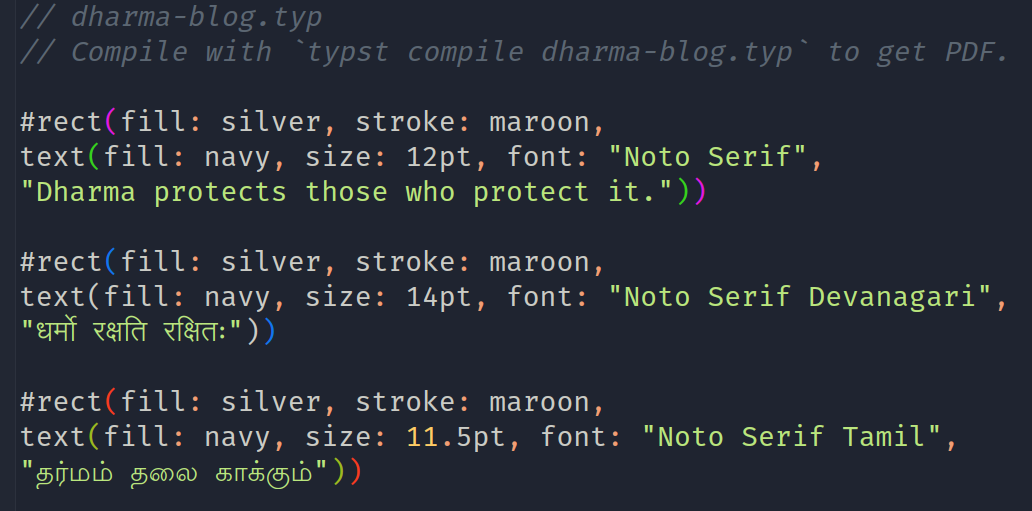
\includegraphics[width=0.9\textwidth,height=\textheight]{images/dharma-source.png}
\caption{Source code in \texttt{Typst} for mottoes in three
languages.}\label{fig:dharma-source}
}
\end{figure}

I think that you would agree with me that the file to accomplish this
multi-lingual, graphically enhanced text is about as concise as it can
be, in order to be complete and self-contained. Moreover, the purpose of
the text in the source file is easily comprehended, even by those
unfamiliar with Typst. The result is shown in \cref{fig:dharma}. If you
are incredulous enough to want to compile the source file for yourself,
to get the PDF, here are the links for
\href{auxiliary/dharma-blog.typ}{source} and
\href{auxiliary/dharma-blog.pdf}{PDF}.\footnote{Of course, you need the
  invoked fonts for successful compilation. If you are interested in
  other languages, whose fonts you do have, you could substitute texts
  in those languages and compile. To find out which fonts are seen by
  Typst, execute \texttt{typst\ fonts} in a terminal. I think you will
  agree that things could not get much simpler.}

\begin{figure}
\hypertarget{fig:dharma}{%
\centering
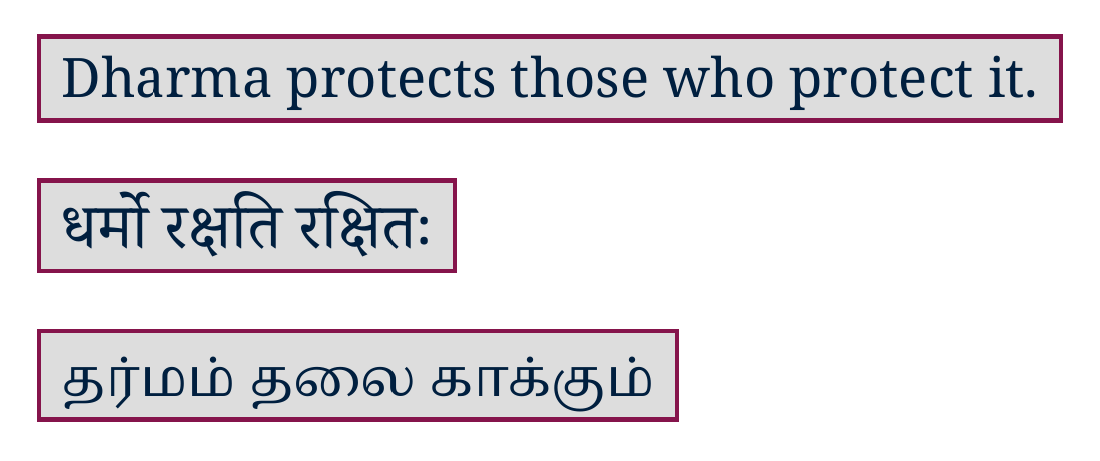
\includegraphics[width=0.7\textwidth,height=\textheight]{images/dharma.png}
\caption{Output from the file \texttt{dharma-blog.typ} after compilation
into a PDF.}\label{fig:dharma}
}
\end{figure}

\hypertarget{available-letter-templates-in-typst}{%
\subsubsection{Available letter templates in
Typst}\label{available-letter-templates-in-typst}}

Let us now return to the main task of writing a letter using Typst.
First, there are
\href{https://github.com/qjcg/awesome-typst\#letters}{ready-made
templates for letters in Typst} that are available on the web. A cursory
glance revealed that these conform to the
\href{https://en.wikipedia.org/wiki/DIN_5008}{DIN 5008 norm} which
introduces a degree of formality that is out of place in a social or
casual letter. Moreover, developing a letter-template from scratch would
reveal how simple or complicated a scripting language Typst is. That is
the route taken here.

\hypertarget{senders-address-at-the-top-right}{%
\subsubsection{Sender's address at the top
right}\label{senders-address-at-the-top-right}}

It is customary, when writing letters in English, to align the sender's
address and the date to the top right of the page and for the
recipient's address to be left-aligned, below that.

Just these two text alignments used to take time and effort to achieve
in LaTeX. And if you had a dual-signatory letter, things got even more
entangled.

Let us see how Typst overcomes these hurdles.

\hypertarget{toward-a-letter-template-in-typst}{%
\subsection{Toward a letter template in
Typst}\label{toward-a-letter-template-in-typst}}

In LaTeX, we usually depend on packages written by others to do the
medium-level lifting for our specific purposes, with simple option-like
customizations left to ourselves. In Typst, we are ourselves empowered
to customize our document, because template development\footnote{Think
  \texttt{documentclass} in LaTeX.} is not as forbidding a task as it is
in LaTeX, which requires a steep learning curve.

The explanations on Typst that I give here might not be exact because I
am a learner myself, and also because Typst itself is evolving. As I
understand it, Typst allows content and its formatting to be specified
in a template that marries the two. This is because the document we are
creating may be structured into the natural components we envisage. In
this sense, \emph{Typst is a document-templating language}.

Once the template is complete, we invoke it much like a
\texttt{\textbackslash{}documentclass} command in LaTeX. But there the
similarity ends. After invoking the template, we fill the content for
each structural element of the document and we produce an
\emph{instantiation} of a letter from the template. Here, \emph{Typst is
a document-markup and typesetting language}. We then \emph{compile} the
letter into a PDF document and view the end result.

If the appearance of any element is amiss in the PDF, we can correct it
at once in the source document and view the result once more. Because
compilation is very fast, we can work interactively in this manner to
get decent results in a short time.

\hypertarget{template-reflects-structure}{%
\subsection{Template reflects
structure}\label{template-reflects-structure}}

The text below is the beginning of the template and embodies the
document structure of a letter:

\begin{figure}
\hypertarget{fig:template}{%
\centering
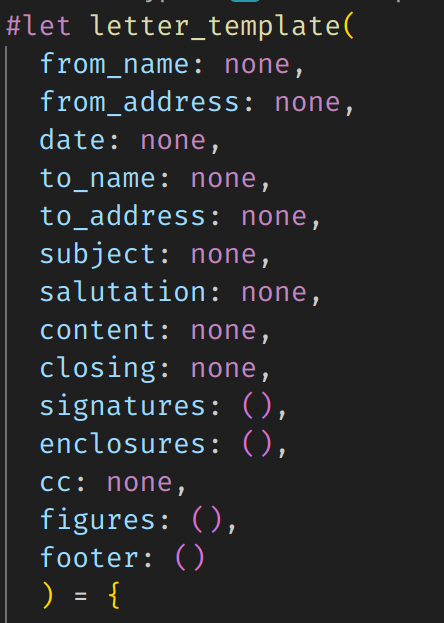
\includegraphics[width=0.5\textwidth,height=\textheight]{images/letter-template-top.png}
\caption{Top of letter template showing the structure of the letter as
fields.}\label{fig:template}
}
\end{figure}

It has the same sequential spatial structure as a letter, starting at
the top and moving to the bottom. All the defined fields have
self-explanatory names. The content of the fields are set to
\texttt{none} because this is a template rather than an instance of a
letter. Fields with \texttt{()} are arrays that will be filled as the
letter is fleshed out. The actual values will be set in the specific
letter we choose to write. The document template is therefore a
\emph{mapping} or set of key-value pairs in which the value is
initialized to \texttt{none}. If we want the template to assume default
values for unchanging fields like \texttt{from\_name},
\texttt{from\_address}, etc., we may set those in the template itself.

Note that at this stage, nothing has been said about page size, text
alignment, font name, etc. All that follows \emph{after} this structure
has been laid out.

\hypertarget{filling-the-template-with-content}{%
\subsection{Filling the template with
content}\label{filling-the-template-with-content}}

When the fields in the template are filled in with content or data, we
have the letter materializing out of the template.

\begin{figure}
\hypertarget{fig:letter}{%
\centering
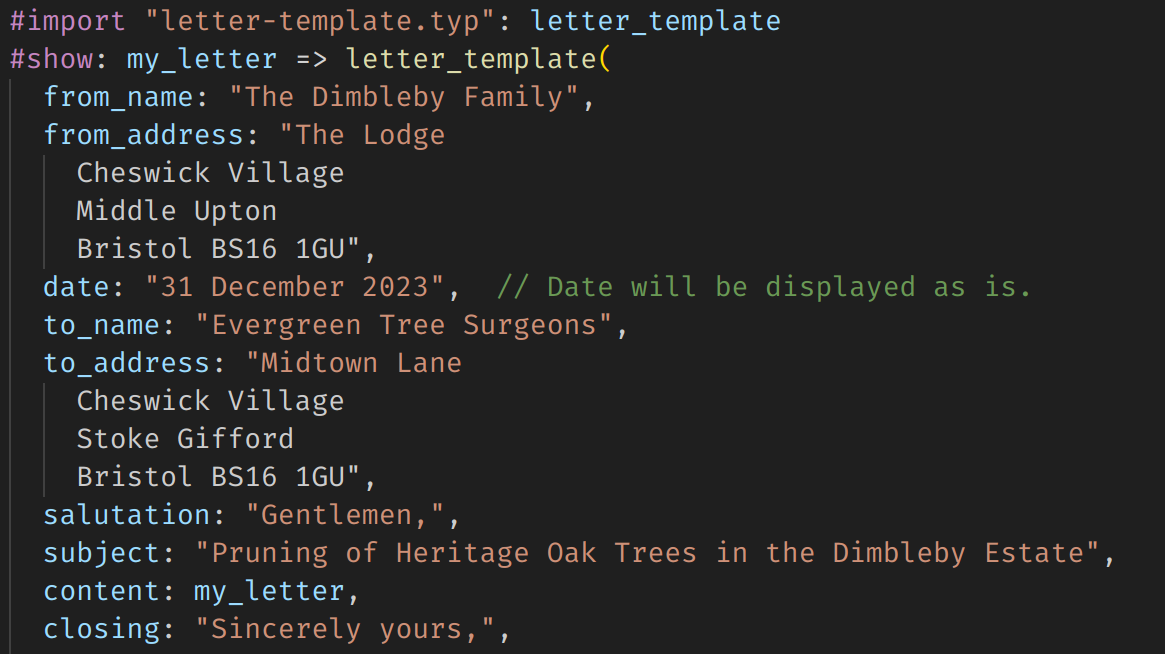
\includegraphics[width=0.98\textwidth,height=\textheight]{images/letter-content-top.png}
\caption{Top of actual letter with content filled in.}\label{fig:letter}
}
\end{figure}

The markup, such as alignment, etc., comes later in the template in the
form of code associated with each element, as shown in \cref{fig:align}:

\begin{figure}
\hypertarget{fig:align}{%
\centering
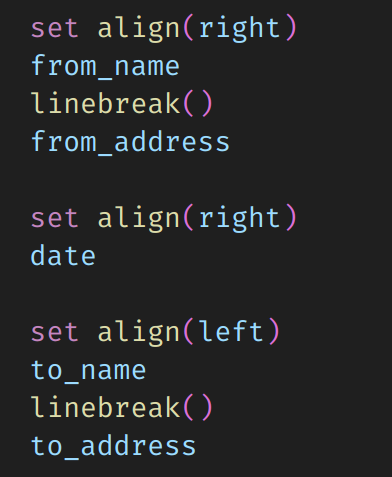
\includegraphics[width=0.4\textwidth,height=\textheight]{images/align-right-left.png}
\caption{Code for aligning the \texttt{from\_name} and
\texttt{from\_address} to the right, and the \texttt{to\_name} and
\texttt{to\_address} to the left.}\label{fig:align}
}
\end{figure}

Note that content appears as strings within double quotes,
\texttt{"...",} or within brackets. \texttt{{[}...{]}}. Because a typst
file accommodates both a programming language and some content in the
same file, we need to adhere to an unambiguous syntax to discriminate
between code and content.

The completed letter is then passed through Typst with the simple
command \texttt{typst\ compile\ \textless{}basename.typ\textgreater{}}.
We then get as output the PDF of the letter we desire. SVG images,
produced by converting the PDF, are shown below, albeit with a
transparent background, which highlights the scanned signatures:

\begin{center}

\includesvg[width=0.47\textwidth,height=\textheight]{images/letter-1.svg}
\includesvg[width=0.47\textwidth,height=\textheight]{images/letter-2.svg}

\end{center}

There are other features in the template that require a little more
explanation, but we will skip them for now, because we are after a proof
of concept that a PDF letter produced by Typst is both of high quality
and also easy to typeset. The three example files we have used are:

\begin{enumerate}
\item
  \href{auxiliary/letter-template.typ}{\texttt{letter-template.typ}}:
  fully commented template file
\item
  \href{auxiliary/letter.typ}{\texttt{letter.typ}}: actual letter file
\item
  \href{auxiliary/letter.pdf}{\texttt{letter.pdf}}: PDF output of letter
\end{enumerate}

Do view the end result,
\href{auxiliary/letter.pdf}{\texttt{letter.pdf}}, in a web browser or
PDF reader.

Feel free to modify and use these files to meet your requirements.

\hypertarget{afterthoughts-on-typst}{%
\subsection{Afterthoughts on Typst}\label{afterthoughts-on-typst}}

If you could view the PDF letter produced with Typst, I hope you were
suitably impressed both by the professional quality of the output, as
well as the simplicity of generating it.

The following embellishments on a normal ``vanilla-flavoured'' letter
are shown in the template:

\begin{enumerate}
\def\labelenumi{\alph{enumi}.}
\item
  Redaction of content by a simple command.
\item
  Multiple signatories, neatly arrayed at the bottom of the letter.
\item
  A footer with contact hyperlinks that gives the letter a more
  business-like tone.
\item
  Addition of fields for cc (carbon copy) and encl (enclosures).
\item
  Ability to seamlessly integrate a captioned image as an enclosure.
\end{enumerate}

Above all, the letter template and letter have demonstrated that a
newcomer to \texttt{Typst} can generate a serviceable template and
produce a PDF letter, within a few hours of encountering Typst.

I have two suggestions for Typst:

\begin{enumerate}
\def\labelenumi{\roman{enumi}.}
\item
  The name \texttt{Typst} seems rather infelicitous to pronounce. At the
  very least there should be an explanation on how to pronounce
  it.\footnote{After finishing this blog, I came across
    \href{https://github.com/typst/typst\#pronunciation-and-spelling}{this
    explanation on how to pronounce \texttt{Typst}}.} If it were
  possible, I myself would vote for a visually less daunting name
  change, though. \emojifont {😉} \normalfont
\item
  If \texttt{Typst} could be harnessed to produce HTML output, either on
  its own, or through \texttt{Pandoc}, we would be on the cusp of a
  typesetting revolution, because ePub would also then be possible with
  a few tweaks, from a single source document.\footnote{After I had
    concluded this blog, I came stumbled upon
    \href{https://github.com/typst/typst/issues/721}{this discussion on
    GitHub} in which HTML export is planned natively from \texttt{Typst}
    source. Hurrah!}
\end{enumerate}

My overall experience using Typst has been very positive. The fact that
I now have a template for letters means that my future letter-writing
tasks will be lightened considerably. Count me in as a recent and
enthusiastic convert to Typst! Long may it flourish!

\hypertarget{acknowledgements}{%
\subsection{Acknowledgements}\label{acknowledgements}}

As a beneficiary of Typst, I thank its creators, Martin Haug and Laurenz
Mädje, for producing a gem of a programmable typesetting system.

I am deeply grateful to my son, Nandakumar Chandrasekhar, for
constructing a generalized letter template in Typst at very short
notice. He found the task pleasantly rewarding, even though he did not
have any prior familiarity with the language.

I thank user 127071 at
\href{https://pixabay.com/photos/storm-damage-oak-tree-break-597217/}{Pixabay}
for generously permitting use of the image in the example letter.

May I also clarify that the contents of the sample letter,
\href{auxiliary/letter.pdf}{\texttt{letter.pdf}}, are entirely the
result of my flights of fancy, and bear no resemblance to any person,
organization, or location. I was having fun imagining things, plain and
simple! \emojifont {😉} \normalfont

\hypertarget{feedback}{%
\subsection{Feedback}\label{feedback}}

Please \href{mailto:feedback.swanlotus@gmail.com}{email me} your
comments and corrections.

\noindent A PDF version of this article is
\href{./using-typst-for-letters.pdf}{available for download here}:

\begin{small}

\begin{sffamily}

\url{https://swanlotus.netlify.app/blogs/using-typst-for-letters.pdf}

\end{sffamily}

\end{small}

\hypertarget{bibliography}{%
\section*{References}\label{bibliography}}
\addcontentsline{toc}{section}{References}

\hypertarget{refs}{}
\begin{CSLReferences}{0}{0}
\leavevmode\vadjust pre{\hypertarget{ref-typst01}{}}%
\CSLLeftMargin{{[}1{]} }%
\CSLRightInline{reknih. 2023. {Typst, a new markup-based typesetting
system, is now open source}. Retrieved 1 January 2024 from
\url{https://news.ycombinator.com/item?id=35250210}}

\leavevmode\vadjust pre{\hypertarget{ref-typst02}{}}%
\CSLLeftMargin{{[}2{]} }%
\CSLRightInline{desperado339. 2023. {Check out Typst, a modern LaTeX
alternative written in Rust}. Retrieved 1 January 2024 from
\url{https://www.reddit.com/r/rust/comments/18001dr/check_out_typst_a_modern_latex_alternative}}

\leavevmode\vadjust pre{\hypertarget{ref-xiang2020}{}}%
\CSLLeftMargin{{[}3{]} }%
\CSLRightInline{Alan Xiang. 2020. {LaTeX3: Programming in LaTeX with
Ease}. Retrieved 1 January 2024 from
\url{https://www.alanshawn.com/tech/2020/10/04/latex3-tutorial.html}}

\leavevmode\vadjust pre{\hypertarget{ref-typstref}{}}%
\CSLLeftMargin{{[}4{]} }%
\CSLRightInline{Martin Haug and Laurenz Mädje. 2023. {typst
Documentation: Reference}. Retrieved 7 January 2024 from
\url{https://typst.app/docs/reference/}}

\end{CSLReferences}



\end{document}
